\chapter{Why Topology?}
\graphicspath{ {/home/tomasp/Dokumenty/Master_Thesis/figures/} }

Data has shape. This is hardly a new or revolutionary idea in the realm of data analysis and statistics. It is an assumption that we make all the time, even if we do not say it out loud. Whenever one tries to construct a linear regression model, we all have the mental image of a straight line in our minds, which should roughly approximate the data. This is then generalized via hyperplanes in higher dimensions.
\par
Another example would be periodic time series or signals -- we all expect to see a ``loop'' of some sort, given a long enough time interval between the measurements, see for example \ref{fig:SeattleWeather}. It isn't much of a stretch to imagine that we could use this loop to try to approximate the period of the time series (something that we will actually do in the following chapters, after introducing the necessary mechanisms).

\begin{figure}[h]
  \caption{Example plot of seasonal temperature changes in Seattle throughout the years.}
  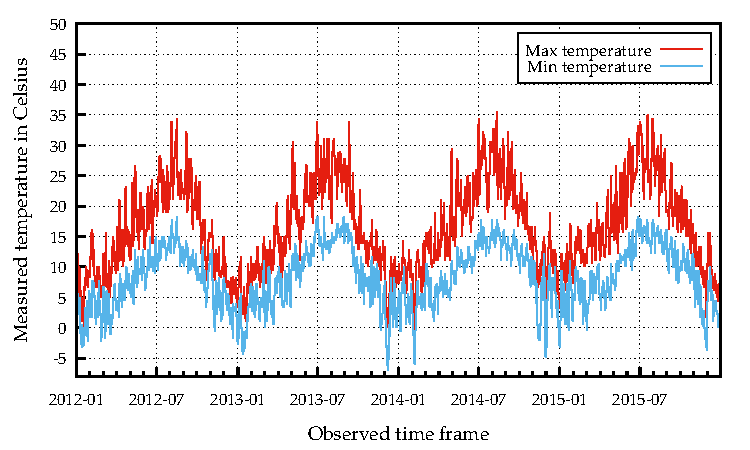
\includegraphics{weather.pdf}
  \centering
  \label{fig:SeattleWeather}
\end{figure}

Clustering algorithms -- be it k-means, hierarchical clustering and so on -- all work with the shape and geometry of our data explicitly by partitioning the available search space into the distinct clusters, once a measure of distance (which doesn't need to be a metric, per se) is chosen. The list could go on, but I believe the point was already made. Historically and traditionally, an appropriate analytic model was derived and constructed for each of the above-mentioned methods with a rich theoretical background to justify the results.
\par
While this approach works for most simple cases the average data analyst will encounter on an Excel spreadsheet, thanks to the advancements made in computing power and software engineering, we're collecting massive amounts of complicated, high-dimensional data living faster than we did before, especially in the fields of biology and medical sciences.

\begin{figure}[h]
  \caption{Time-scaled phylogenetic tree of H3 influenza viruses inferred by BEAST using molecular clock model.}
  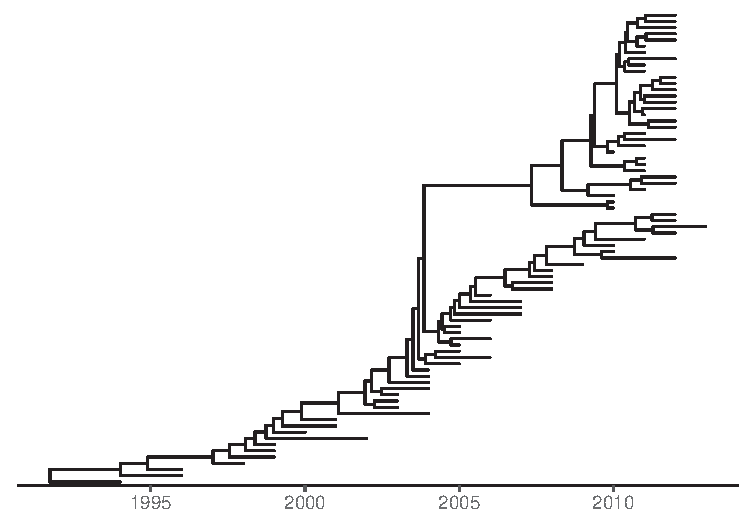
\includegraphics{influenzaTree.pdf}
  \centering
  \label{fig:influenzaTree}
\end{figure}

A good example of that would be phylogenetic and evolutionary trees, like the one in \ref{fig:influenzaTree}. We might be interested to know whether any mutation occurred, where did they happen and how far were they transmitted down the tree. We might look for re-combinations of the genomic material or both horizontal and vertical transfer of it. All those questions pertain to the shape of the phylogenetic tree and its branching.\
\footnote{Data downloaded from \href{https://datadryad.org/stash/dataset/doi:10.5061/dryad.v15v0}{the following link},
visited on the 01.08.2024}
\par
The situation only gets more complex with each passing day and batch of collected data. One \textit{could} try to develop analytical models for each case, provide the rigorous theory and obtain the conclusions that they seek. But a far more reasonable and general method would be to instead study the shape itself and approximate the datasets by selecting the shape that describes it the ``best''. This is where topology comes into play, as this gives us the tools and theory to do exactly that, with the help of algebraic topology.
\par
Algebraic topology will help us to qualitatively distinguish the two situations in \ref{fig:Blobs}, where even on an intuitive level we can see that the difference lies in the number of ``blobs'' in each figure; or more rigorously in the number of connected components.

\begin{figure}[h]
  \centering
  \subfloat[\centering 3 blobs]{{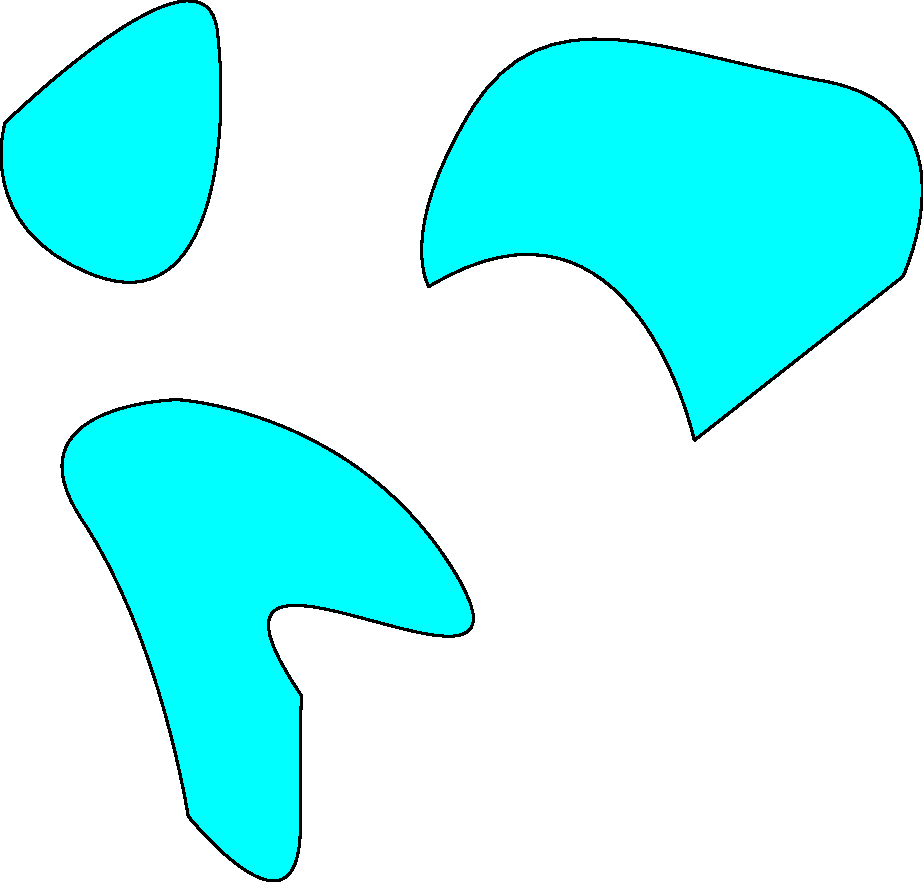
\includegraphics[width=5cm]{blobs_3.pdf} }}%
  \qquad
  \subfloat[\centering 5 blobs]{{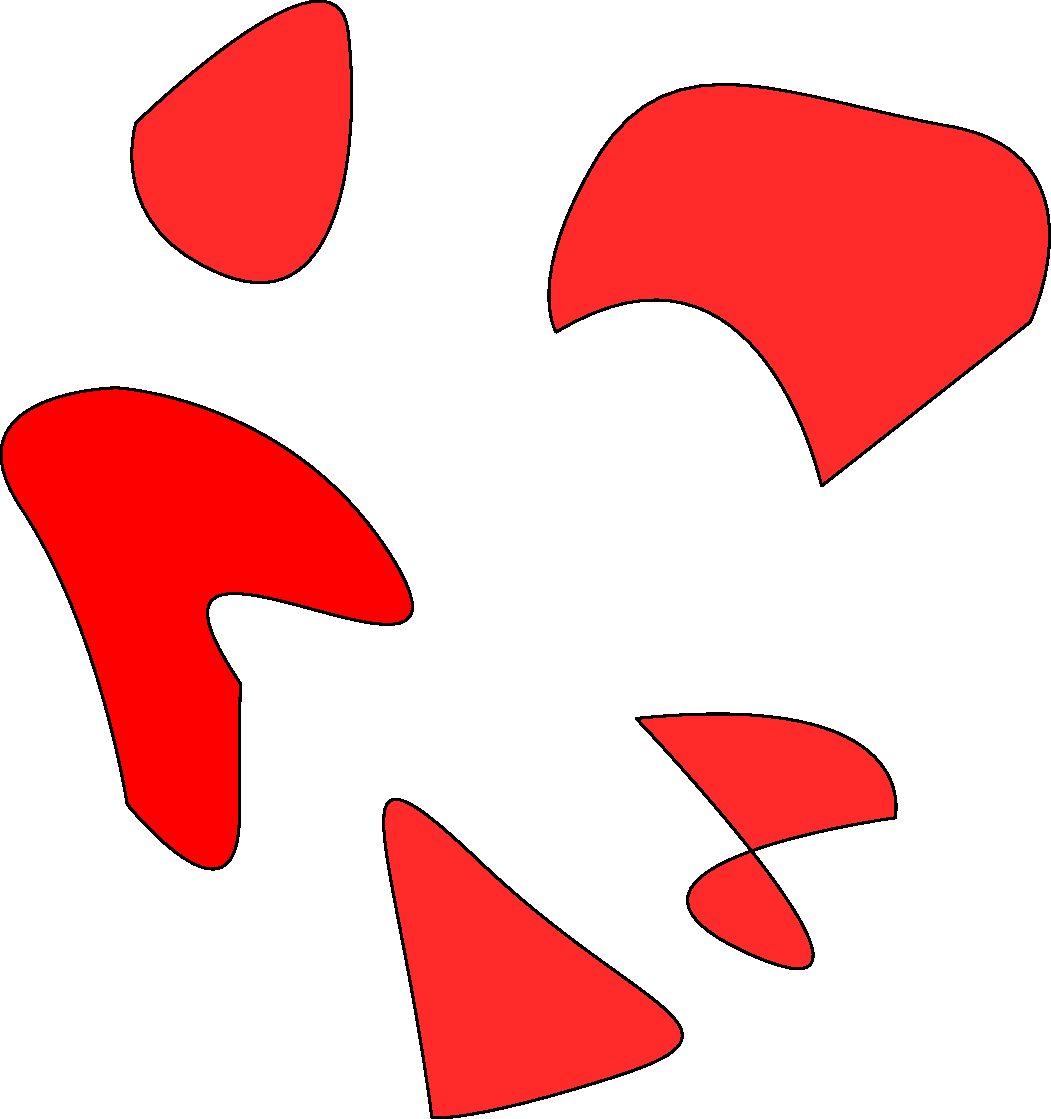
\includegraphics[width=5cm]{blobs_5.pdf} }}%
  \caption{Counting the number of blobs in each figure.}
  \label{fig:Blobs}
\end{figure}

Likewise, using the already established machinery, we will be able to describe and quantify the fact that in \ref{fig:unit_circle} there is a hole in the middle of it.

\begin{figure}[h]
  \caption{Data sampled from a unit circle characterized by the distinct hole in the middle.}
  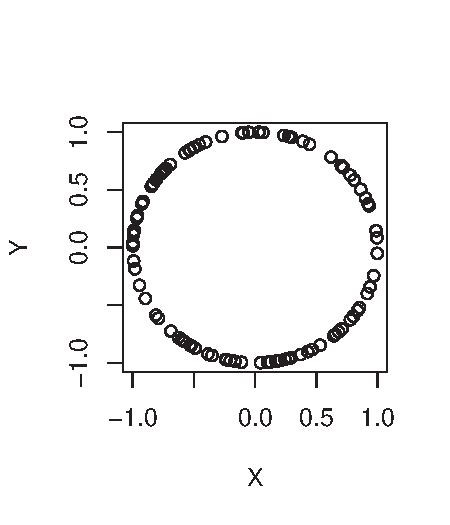
\includegraphics[width=7cm, height=7cm]{unit_circle.pdf}
  \centering
  \label{fig:unit_circle}
\end{figure}

Both of these can be thought of as counting $n-$dimensional holes: connected components being of dimension $0$, while the hole in \ref{fig:unit_circle} is a $1-$dimensional one. We will see how this approach and its extension will be the foundation of what we call TDA -- Topological Data Analysis.
